\documentclass[12pt]{article}

\usepackage{sbc-template}
\usepackage{graphicx,url}
\usepackage{booktabs}
\usepackage[utf8]{inputenc}
\usepackage[T1]{fontenc}
\usepackage[english]{babel}

\graphicspath{{../reports/figures/}{reports/figures/}}

\sloppy

% TODO: replace with the final title (research question: do structural
% characteristics of a school predict the average ENEM 2025 performance of its students?)
\title{Do School Characteristics Predict ENEM Performance? A Grouped and Nested
  Evaluation of Regression Models on Brazilian High Schools}

\author{Artur Mariano da Silva\inst{1}, Emerson Herrera\inst{1}, Yaser Husein\inst{1}}

\address{Instituto de Informática -- Universidade Federal do Rio Grande do Sul (UFRGS)\\
  Porto Alegre -- RS -- Brazil
  \email{\{artur.mariano,TODO-email-2,TODO-email-3\}@inf.ufrgs.br}
}

\begin{document}

\maketitle

\begin{abstract}
  % TODO: abstract (max. 10 lines, first page): problem, data (ENEM 2025 + School Census 2024),
  % method (grouped repeated CV, spot-checking, nested CV), main result, interpretation.
  
We investigate to what extent the structural characteristics of Brazilian high schools predict the average ENEM 2025 score of their students. Joining the ENEM 2025 results with the Censo  Escolar 2024, we build a data set of 23{,}374 schools described by 45 attributes of
  infrastructure, size, network, and location. Six regression algorithms are compared with
  cross-validation grouped by municipality and repeated three times, followed by nested
  cross-validation for hyperparameter tuning and the Friedman and Nemenyi tests. A tuned gradient
  boosting model reaches an RMSE of 30.6 points ($R^2 = 0.76$), statistically tied with SVR,
  against 39.7 points when only the administrative network is known. SHAP values and ablations
  show that the network dominates the predictions, but the remaining structural attributes still
  explain $R^2 = 0.64$ without it.
\end{abstract}

\section{Introduction}
\label{sec:introduction}

% TODO (group writes the text). Cover: context of ENEM and school-level inequality; the research
% question (do structural characteristics of a school -- infrastructure, administrative network,
% location, size, teaching staff -- predict the average ENEM 2025 score of its students?);
% why regression at school level; contributions; paper outline.
% Source of facts: ../README.md. Citations come from the references task (T17).

\section{Related Work}
\label{sec:related-work}

% TODO (group writes the text). Cover: prior work on predicting educational performance from
% school/socioeconomic factors (ENEM, INEP data, school effects); ML for educational data mining;
% model comparison methodology (repeated CV, Friedman/Nemenyi) and SHAP-based interpretation.
% Only cite verified references from references.bib (T17).

\section{Data and Exploratory Analysis}
\label{sec:data}

% TODO (group writes the text). Cover:
% - Sources: ENEM 2025 microdata and School Census 2024 (INEP); include the DATASET DOWNLOAD LINK
%   (required by the assignment). URLs and SHA-256 of each source are in the metadata JSON
%   generated by scripts/build_dataset.py (data/processed/*.json).
% - Unit of analysis: school with >= 10 candidates present in all 4 tests; target nota_media
%   (mean over schools of the mean of the 5 scores). Number of schools and attributes (README.md).
% - EDA findings required by the assignment: attribute types/quantity, target distribution,
%   patterns, anomalies (88888 code, 15 schools), missing values, scale, outliers, inconsistencies.
%   Source: ../reports/eda.md.
% - Figures below: choose which to keep (page limit is 20 pages including references).

\subsection{Sources and construction of the data set}

Two public data sets published by INEP were used: the ENEM 2025 microdata
\cite{inep2025enem}, file \texttt{RESULTADOS\_2025.csv}, available at
\url{https://download.inep.gov.br/microdados/microdados_enem_2025.zip}, and the Censo Escolar
2024 microdata \cite{inep2024censo}, available at
\url{https://download.inep.gov.br/dados_abertos/microdados_censo_escolar_2024.zip}. The 2024
census was selected because the 2025 edition had not been published when the data were collected; the
structural characteristics of a school change slowly, so the one-year lag should have little
effect, but we return to it in Section~\ref{sec:conclusion}.

A candidate is kept only if present in the four ENEM tests, with the five scores (natural
sciences, human sciences, languages, mathematics, and essay) and a school code. This leaves
1{,}288{,}485 candidates in 29{,}341 schools. For each candidate we take the mean of the five
scores, and for each school the mean over its candidates; this school mean, \texttt{nota\_media},
is the target. We keep schools with at least ten valid candidates (23{,}570 schools), so that the
target is not dominated by a handful of students, and join them with the census by school code.
The final table has \textbf{23{,}374 schools} (99.2\% of the schools above the threshold) in
5{,}201 municipalities.

Each school is described by 45 attributes from the census, chosen to represent what a school or
an education department can act upon: 31 binary infrastructure indicators (\texttt{IN\_*}, e.g.,
science laboratory, library, internet for students, school meals), 9 counts of size and resources
(\texttt{QT\_*}, e.g., high-school enrolment, teachers, rooms, computers), and 5 categorical
attributes of network and location (administrative network \texttt{TP\_DEPENDENCIA}, urban/rural
location, differentiated location, region, and state). The municipality code is used only to
define the cross-validation groups (Section~\ref{sec:methodology}) and is never a model input.


\begin{figure}[ht]
  \centering
  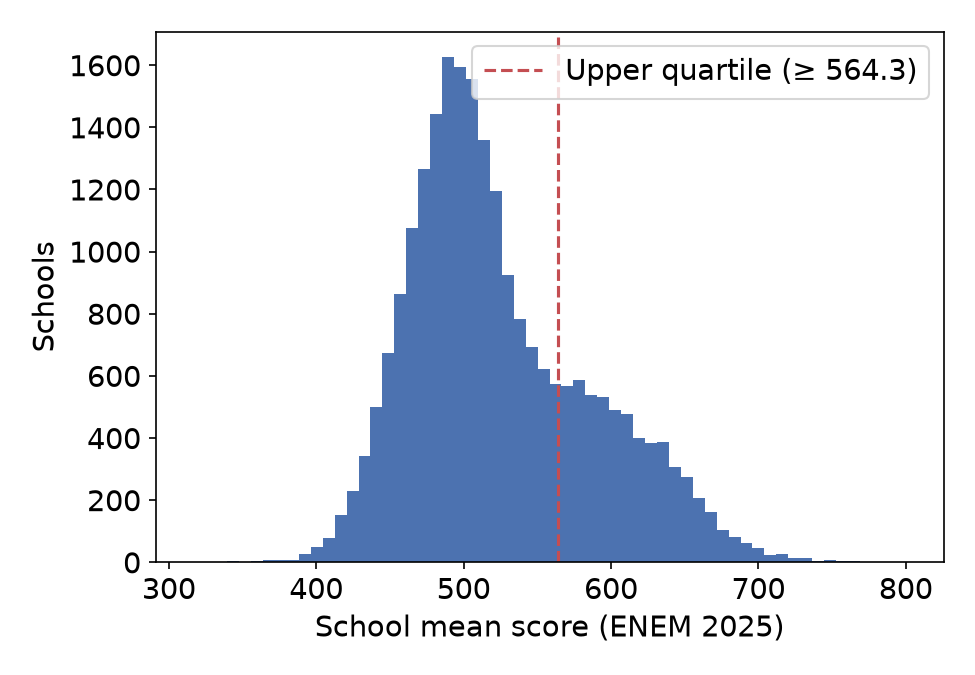
\includegraphics[width=0.7\textwidth]{target_hist.png}
  \caption{TODO: caption -- distribution of the target (\texttt{nota\_media}).}
  \label{fig:target-hist}
\end{figure}

\begin{figure}[ht]
  \centering
  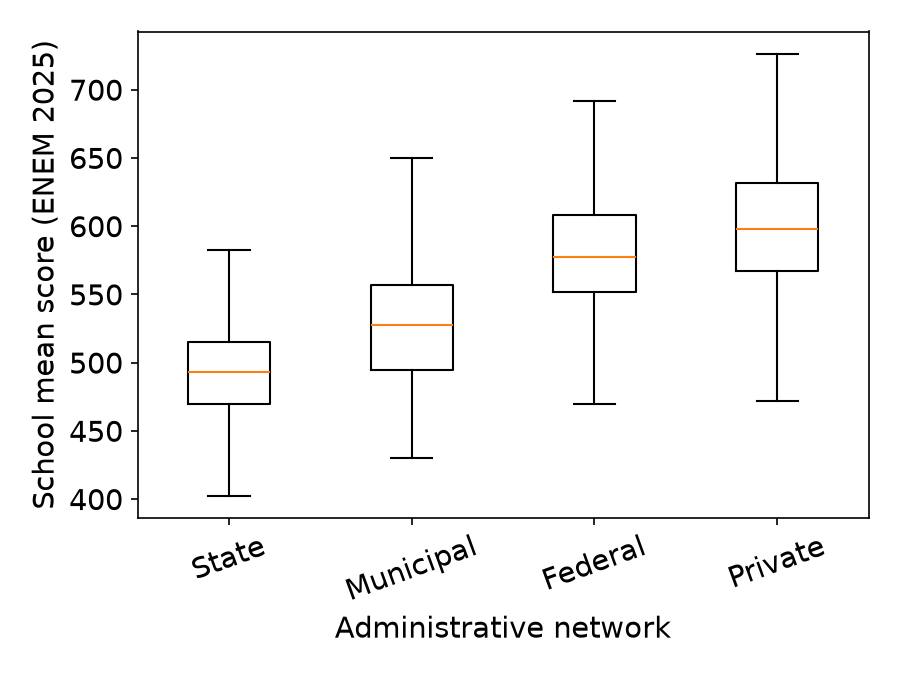
\includegraphics[width=0.7\textwidth]{target_by_dependencia.png}
  \caption{TODO: caption -- target by administrative network.}
  \label{fig:target-dependencia}
\end{figure}

\begin{figure}[ht]
  \centering
  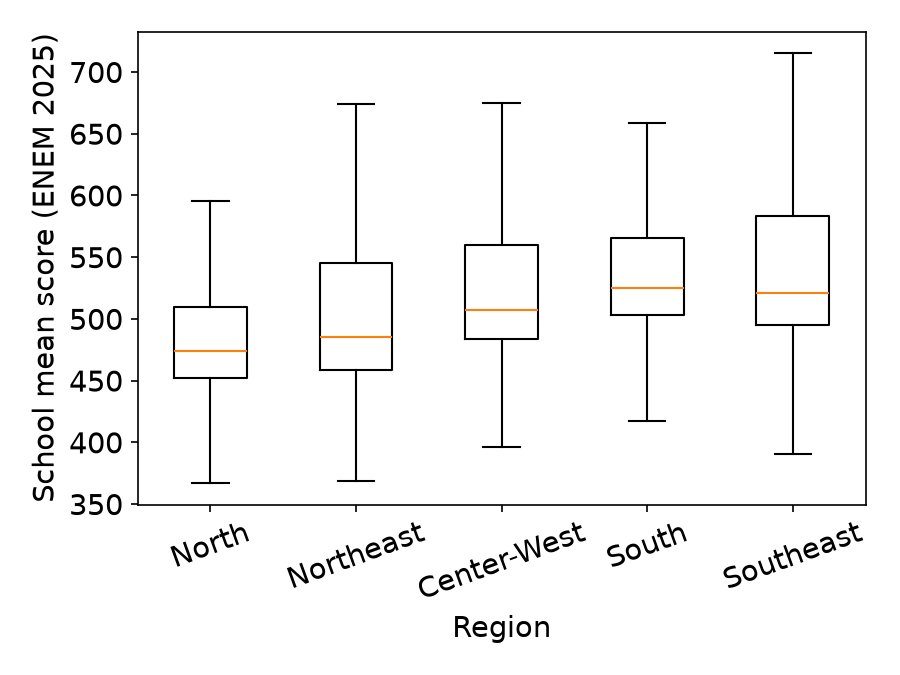
\includegraphics[width=0.7\textwidth]{target_by_regiao.png}
  \caption{TODO: caption -- target by region.}
  \label{fig:target-regiao}
\end{figure}

% Optional figures available in ../reports/figures/: feature_target_spearman.png,
% count_features_hist.png, target_std_by_school_size.png.

\section{Methodology}
\label{sec:methodology}

% TODO (group writes the text). Subsections suggested:
%
\subsection{Preprocessing}
% 88888 -> missing + indicator; median / most-frequent imputation; log1p + StandardScaler on counts;
% one-hot for categoricals; CO_REGIAO and QT_TUR_MED dropped; everything inside a scikit-learn
% Pipeline fitted only on training folds (no leakage). Code: src/enem_school/preprocessing.py.
%
% \subsection{Grouped cross-validation by municipality}
% GroupKFold by municipality, fixed seed 42; why grouping (schools of the same municipality are
% not independent). Code: assign_folds.
%
% \subsection{Repeated 3x5 evaluation}
% 3 repetitions of 5 folds, same partitions for all algorithms in each iteration (assignment
% requirement); metrics RMSE, MAE, R^2.
%
% \subsection{Spot-checking}
% 6 algorithms with default hyperparameters + baselines (mean; administrative network).
% Notebook: notebooks/02_spot_checking.ipynb.
%
% \subsection{Hyperparameter tuning with nested CV}
% Outer = same grouped 3x5 folds; inner = GroupKFold(3) by municipality; GridSearchCV over small
% grids for tree, SVR, Random Forest, Gradient Boosting; discarded configs (e.g. SVR C=100,
% 137 s/fit). Notebook: notebooks/03_otimizacao.ipynb. Code: src/enem_school/evaluation.py.
%
% \subsection{Statistical comparison}
% Friedman test + Nemenyi post-hoc (critical difference); describe the setup used.

\section{Results}
\label{sec:results}

\subsection{Baselines and linear regression}

Table~\ref{tab:linear} gives the reference points. Predicting the mean gives an RMSE of 62.4
points, the standard deviation of the target. Knowing only the administrative network already
reduces it to 39.7 points ($R^2 = 0.59$). The linear regression with all the attributes
(variant~A) reaches 34.3 points ($R^2 = 0.70$), so the structural attributes add 5.4 points over
the network alone. Relative to state schools, and conditional on the other attributes, the linear
model adds 84.2 points to private schools, 60.4 to federal schools, and 21.8 to municipal schools.

\begin{table}[htbp]
  \centering
  \caption{Baselines and linear regression variants: mean $\pm$ standard deviation over the five
    folds of the first grouped partition.}
  \label{tab:linear}
  \resizebox{\textwidth}{!}{\begin{tabular}{llll}
\toprule
Model & RMSE & MAE & $R^2$ \\
\midrule
Baseline: mean & 62.41 $\pm$ 1.63 & 50.25 $\pm$ 1.36 & -0.00 $\pm$ 0.00 \\
Baseline: network & 39.73 $\pm$ 1.04 & 30.73 $\pm$ 0.88 & 0.59 $\pm$ 0.00 \\
Linear A (with network) & 34.32 $\pm$ 0.93 & 26.15 $\pm$ 0.54 & 0.70 $\pm$ 0.01 \\
Linear B (without network) & 37.40 $\pm$ 0.81 & 28.30 $\pm$ 0.55 & 0.64 $\pm$ 0.01 \\
Linear C (without network and school meals) & 43.97 $\pm$ 1.34 & 33.63 $\pm$ 0.93 & 0.50 $\pm$ 0.01 \\
\bottomrule
\end{tabular}
}
\end{table}

\subsection{Spot-checking}

Table~\ref{tab:spot} and Figure~\ref{fig:spot} summarize the spot-checking over the 15 grouped
partitions. All the algorithms improve on the mean baseline. The SVR (30.77), the random forest
(30.99), and gradient boosting (31.65) lead, followed by $k$-NN (33.91) and linear regression
(34.24); the unpruned decision tree overfits and is the worst model (43.51). The standard
deviations across partitions, about one point, are small compared with the differences between
the groups of algorithms. The Friedman test rejects the hypothesis that all the algorithms are
equivalent ($\chi^2_F = 73.10$, $p = 2.3 \times 10^{-14}$). The average ranks are 1.07 (SVR),
1.93 (random forest), 3.00 (gradient boosting), 4.20 ($k$-NN), 4.80 (linear), and 6.00 (tree),
and the Nemenyi critical difference is 1.95 (Figure~\ref{fig:cd}). The SVR and the random forest are therefore better
than $k$-NN, linear regression, and the tree, and gradient boosting is better than the tree; the
three leaders cannot be separated from one another.

Since the three leaders are statistically tied, and default hyperparameters can hide an algorithm
that would improve more with tuning, we took all three to the tuning stage instead of only the
top-ranked one. We also tuned the decision
tree, whose poor result was clearly caused by the lack of pruning rather than by the algorithm
itself. The training times per fold (6.5~s for the SVR, 2.2~s for gradient boosting, and 1.1~s for
the random forest, on a 12-core machine) made the nested search feasible for the four algorithms.

\begin{table}[htbp]
  \centering
  \caption{Spot-checking with default hyperparameters: mean $\pm$ standard deviation over the
    $3 \times 5$ grouped partitions, and mean training time per fold.}
  \label{tab:spot}
  \begin{tabular}{llllr}
\toprule
Model & RMSE & MAE & $R^2$ & Train time (s) \\
\midrule
SVR & 30.77 $\pm$ 0.90 & 23.43 $\pm$ 0.62 & 0.76 $\pm$ 0.01 & 6.49 \\
Random Forest & 30.99 $\pm$ 0.90 & 23.63 $\pm$ 0.68 & 0.75 $\pm$ 0.01 & 1.05 \\
Gradient Boosting & 31.65 $\pm$ 0.95 & 24.19 $\pm$ 0.70 & 0.74 $\pm$ 0.01 & 2.20 \\
kNN & 33.91 $\pm$ 1.08 & 25.82 $\pm$ 0.78 & 0.70 $\pm$ 0.01 & 0.03 \\
Linear & 34.24 $\pm$ 1.15 & 26.10 $\pm$ 0.82 & 0.70 $\pm$ 0.01 & 0.04 \\
Decision Tree & 43.51 $\pm$ 1.04 & 33.38 $\pm$ 0.67 & 0.51 $\pm$ 0.02 & 0.18 \\
Baseline: mean & 62.35 $\pm$ 1.85 & 50.20 $\pm$ 1.45 & -0.01 $\pm$ 0.01 & 0.03 \\
\bottomrule
\end{tabular}

\end{table}

\begin{figure}[htbp]
  \centering
  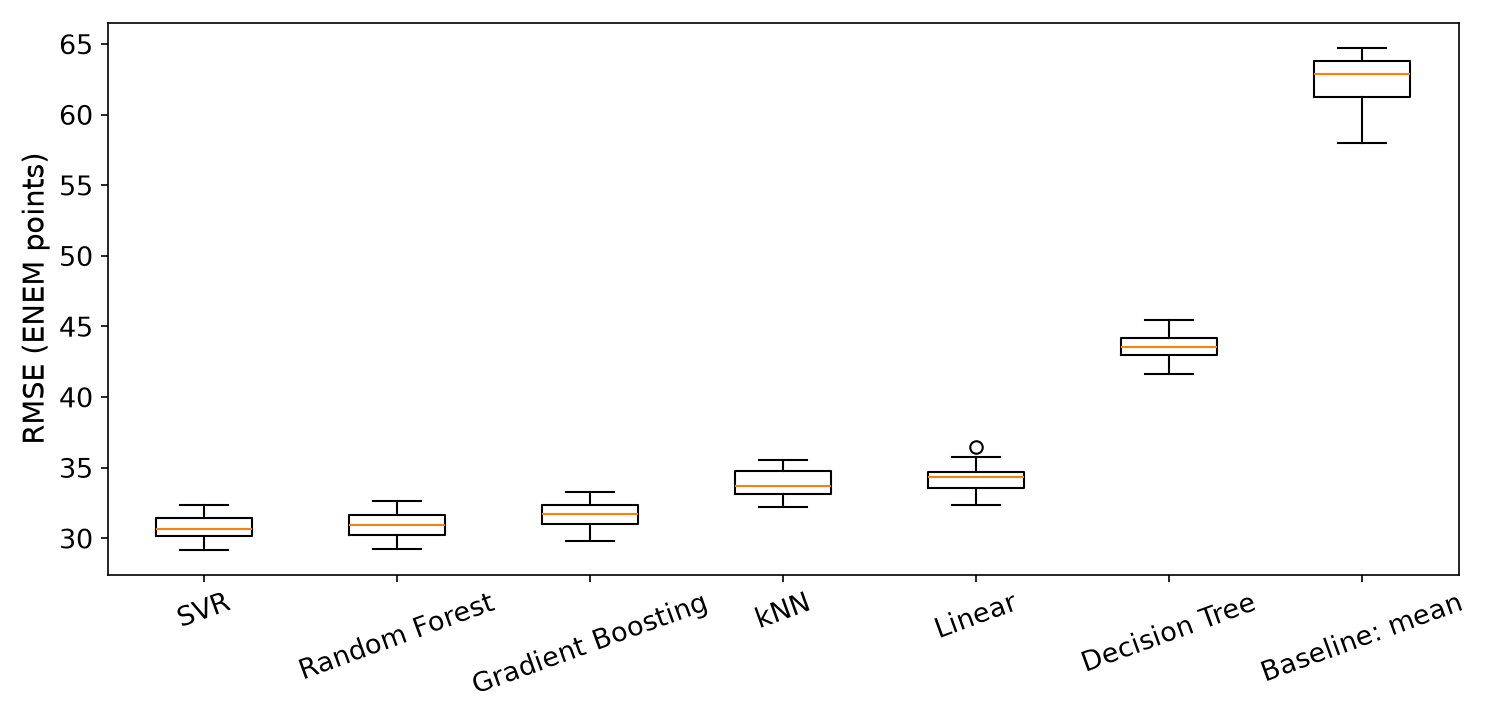
\includegraphics[width=0.9\textwidth]{spot_checking_rmse.png}
  \caption{RMSE of each algorithm over the 15 grouped partitions of the spot-checking.}
  \label{fig:spot}
\end{figure}

\begin{figure}[htbp]
  \centering
  \resizebox{\linewidth}{!}{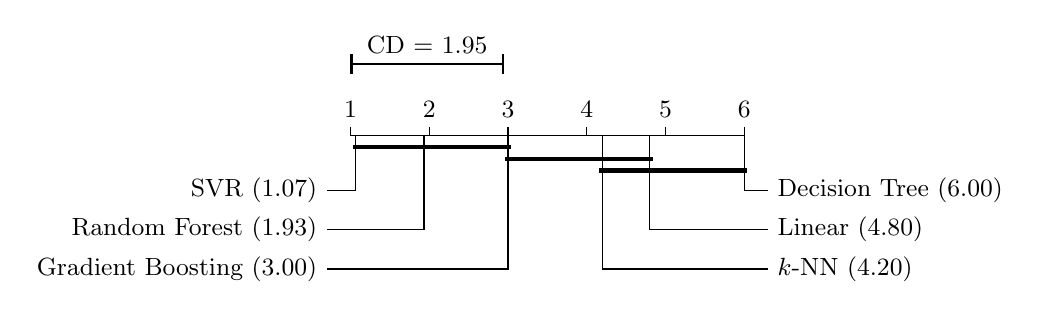
\begin{tikzpicture}[x=1cm,y=1cm,font=\small]
\draw (0,0) -- (5.0,0);
\draw (0.0,0) -- (0.0,0.1) node[above]{1};
\draw (1.0,0) -- (1.0,0.1) node[above]{2};
\draw (2.0,0) -- (2.0,0.1) node[above]{3};
\draw (3.0,0) -- (3.0,0.1) node[above]{4};
\draw (4.0,0) -- (4.0,0.1) node[above]{5};
\draw (5.0,0) -- (5.0,0.1) node[above]{6};
\draw[|-|,thick] (0,0.9) -- (1.947,0.9) node[midway,above]{CD = 1.95};
\draw (0.067,0) -- (0.067,-0.70) -- (-0.3,-0.70) node[left]{SVR (1.07)};
\draw (0.933,0) -- (0.933,-1.20) -- (-0.3,-1.20) node[left]{Random Forest (1.93)};
\draw (2.0,0) -- (2.0,-1.70) -- (-0.3,-1.70) node[left]{Gradient Boosting (3.00)};
\draw (3.2,0) -- (3.2,-1.70) -- (5.3,-1.70) node[right]{$k$-NN (4.20)};
\draw (3.8,0) -- (3.8,-1.20) -- (5.3,-1.20) node[right]{Linear (4.80)};
\draw (5.0,0) -- (5.0,-0.70) -- (5.3,-0.70) node[right]{Decision Tree (6.00)};
\draw[line width=1.6pt] (0.03,-0.15) -- (2.04,-0.15);
\draw[line width=1.6pt] (1.96,-0.30) -- (3.84,-0.30);
\draw[line width=1.6pt] (3.16,-0.45) -- (5.04,-0.45);
\end{tikzpicture}
}
  \caption{Critical-difference diagram of the spot-checking (average ranks over 15 partitions,
    lower is better). Algorithms joined by a bar are not significantly different (Nemenyi,
    $\alpha = 0.05$).}
  \label{fig:cd}
\end{figure}

\subsection{Tuned models}

Table~\ref{tab:tuned} compares the default and tuned versions on the same outer partitions. The
tuning fixes the overfitting of the decision tree, whose RMSE drops by 10.2 points, to 33.31, with
\texttt{max\_depth}$=10$ in all 15 searches. The SVR and the random forest barely change (less than
0.1 point), indicating that their defaults were already close to the best of the grid. Gradient
boosting gains 1.0 point and becomes the best model, with RMSE 30.63 ($R^2 = 0.757$).

\begin{table}[htbp]
  \centering
  \caption{Default vs.\ tuned hyperparameters (nested cross-validation): mean over the
    $3 \times 5$ outer grouped partitions. ``Gain'' is the reduction in RMSE points.}
  \label{tab:tuned}
  \resizebox{\textwidth}{!}{\begin{tabular}{lrrrrrr}
\toprule
Model & RMSE default & RMSE tuned & Std (tuned) & $R^2$ default & $R^2$ tuned & Gain (RMSE) \\
\midrule
Gradient Boosting & 31.654 & 30.634 & 0.898 & 0.741 & 0.757 & 1.020 \\
SVR & 30.770 & 30.676 & 0.892 & 0.755 & 0.756 & 0.094 \\
Random Forest & 30.989 & 30.905 & 0.893 & 0.751 & 0.753 & 0.084 \\
Decision Tree & 43.514 & 33.313 & 0.884 & 0.510 & 0.713 & 10.201 \\
\bottomrule
\end{tabular}
}
\end{table}

The selected hyperparameters were stable: gradient boosting chose \texttt{learning\_rate}$=0.05$
and \texttt{max\_depth}$=5$, and the SVR chose $C=1$ and $\varepsilon=0.3$, in all 15 outer folds;
the random forest chose \texttt{max\_depth}$=20$ in all 15, with \texttt{min\_samples\_leaf}$=1$ in
12. Some of these choices lie on the border of the grid (the smallest learning rate and largest
depth for gradient boosting, the smallest $C$ and largest $\varepsilon$ for the SVR), so a wider
grid could improve them further.

The Friedman test again rejects the null hypothesis ($\chi^2_F = 37.64$, $p = 3.4 \times
10^{-8}$). The average ranks are 1.40 (gradient boosting), 1.73 (SVR), 2.87 (random forest), and
4.00 (tree), with a critical difference of 1.21: gradient boosting and the SVR are better than the
tree, and gradient boosting is better than the random forest, but gradient boosting and the SVR
cannot be separated. In absolute terms, the three best models are within 0.3 RMSE points of each
other, a difference that is small on the ENEM scale. We selected gradient boosting for the
interpretation because it has the lowest error and the best average rank, and because tree
ensembles admit exact and fast SHAP values, which the SVR does not. The whole nested
cross-validation took about 17 minutes.
\section{Interpretation}
\label{sec:interpretation}

% TODO (group writes the text). Cover (notebooks/04_interpretacao.ipynb):
% - SHAP of the tuned Gradient Boosting: global importance (reports/results/shap_importance.csv,
%   Figure~\ref{fig:shap}) and what the main attributes mean.
% - Variants A/B/C (with administrative network / without / without network and school meals):
%   Table~\ref{tab:variants}, source reports/results/interpretacao_variantes.csv.
% - Residual analysis by network x region (Figure~\ref{fig:resid}), e.g. federal schools
%   over/under-predicted by region.
% - Linear model coefficients and residuals if useful: linreg_coefficients.png, linreg_residuals.png.
% - Limitations: structural features are proxies of socioeconomic status; no causal claim.

\begin{figure}[ht]
  \centering
  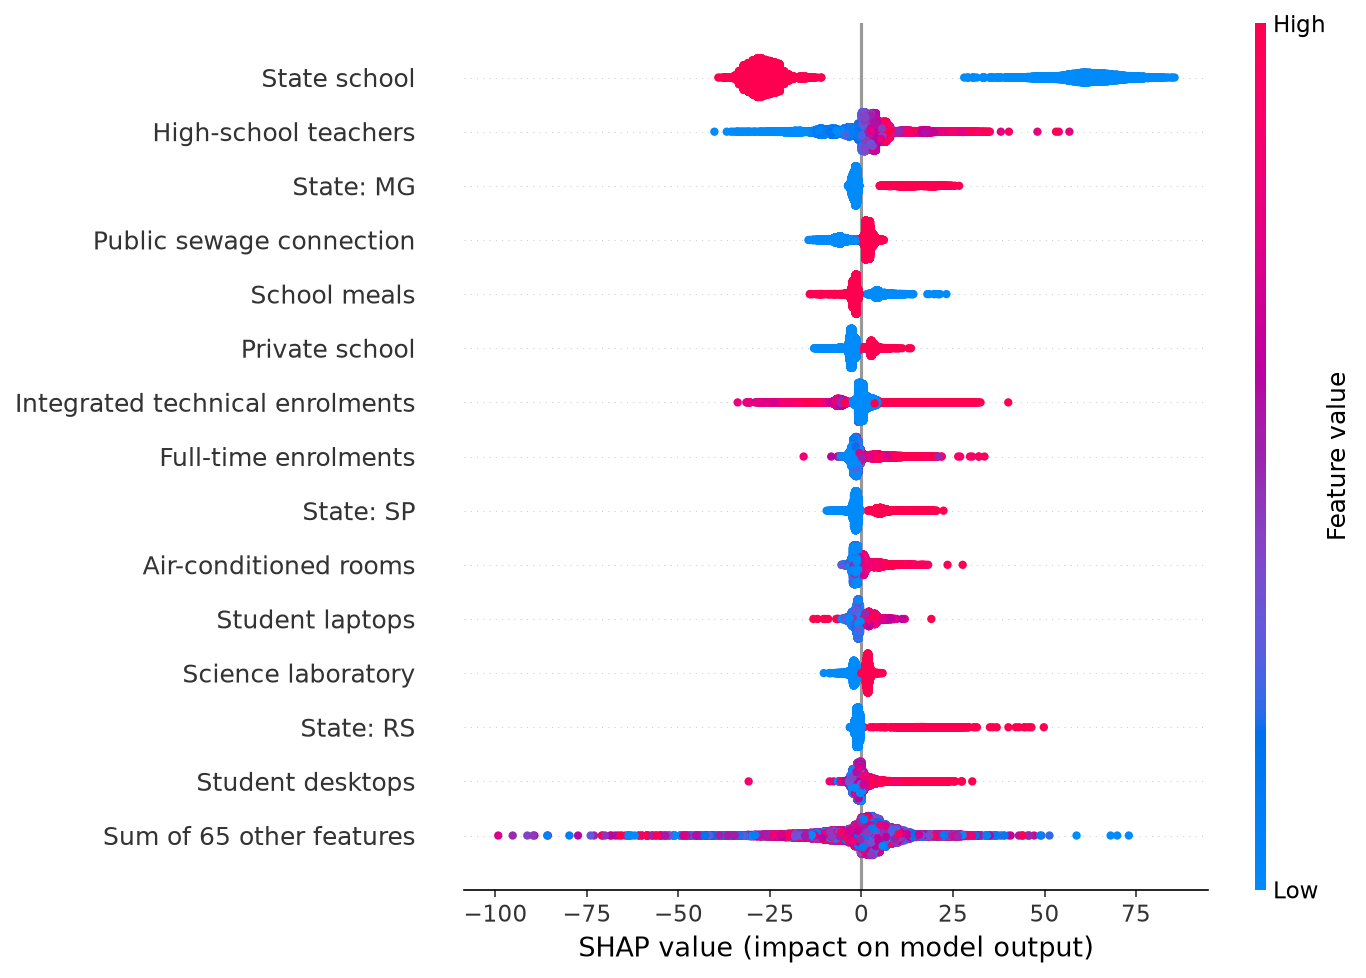
\includegraphics[width=0.8\textwidth]{shap_beeswarm.png}
  \caption{TODO: caption -- SHAP summary (beeswarm) of the tuned Gradient Boosting.}
  \label{fig:shap}
\end{figure}

\begin{table}[ht]
  \centering
  \caption{TODO: caption -- feature-set variants A/B/C, Gradient Boosting vs.\ linear regression.}
  \label{tab:variants}
  \begin{tabular}{llll}
\toprule
Variant & Model & RMSE & $R^2$ \\
\midrule
A & Gradient Boosting & 30.63 $\pm$ 0.90 & 0.76 $\pm$ 0.01 \\
A & Linear & 34.24 $\pm$ 1.15 & 0.70 $\pm$ 0.01 \\
B & Gradient Boosting & 32.46 $\pm$ 1.12 & 0.73 $\pm$ 0.01 \\
B & Linear & 37.32 $\pm$ 1.34 & 0.64 $\pm$ 0.01 \\
C & Gradient Boosting & 37.37 $\pm$ 1.35 & 0.64 $\pm$ 0.01 \\
C & Linear & 43.94 $\pm$ 1.53 & 0.50 $\pm$ 0.02 \\
\bottomrule
\end{tabular}

\end{table}

\begin{figure}[ht]
  \centering
  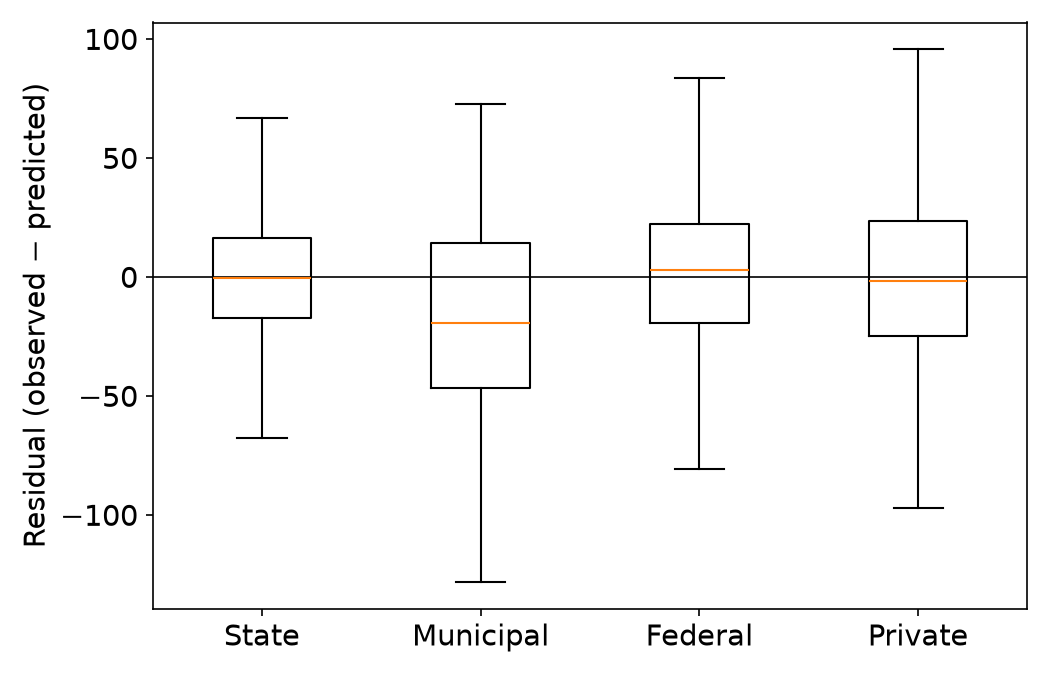
\includegraphics[width=0.8\textwidth]{interpretacao_residuos.png}
  \caption{TODO: caption -- residuals by administrative network and region.}
  \label{fig:resid}
\end{figure}

\section{Reproducibility}
\label{sec:reproducibility}

% TODO (group writes the text; required by the assignment). Cover:
% - Public repository URL (emersonheto/enem-school-performance) and commit/tag of the submission.
% - Data: download link and SHA-256 of each source (metadata JSON from scripts/build_dataset.py).
% - Environment: uv + uv.lock (exact versions), Python 3.12, seeds (SEED = 42, repetition seeds
%   SEED + repeat), fixed folds by municipality.
% - Commands to regenerate: build_dataset.py, eda.py, notebooks 01--04, tests (pytest).
% - Runtime (e.g. nested CV ~17 min) and hardware, if relevant.
% - Models/results shared: reports/results/*.csv.

\section{Conclusion}
\label{sec:conclusion}

% TODO (group writes the text). Cover: answer to the research question with the key numbers
% (best tuned model, gain over baselines, effect of removing network/meals variants), limitations
% (grid borders, proxy variables, school-level aggregation, single ENEM year), future work.

\section*{Use of AI Tools}
\label{sec:ai-use}

During the preparation of this work, the authors utilized the Claude large language model (Anthropic) as an auxiliary tool for two purposes: (i) assisting in code generation and refactoring during the implementation of the predictive modeling pipeline, and (ii) supporting the drafting and improving the readability of the manuscript. All methodological, architectural, and analytical decisions were made exclusively by the authors. Every piece of code and text generated with the assistance of this tool underwent thorough human review, validation, and necessary modifications prior to integration, and the authors take full responsibility for the technical accuracy, originality, and integrity of the publication.

% TODO (group writes the text; required by the assignment: AI use is allowed as support but must
% be cited in the article). State which tools/models were used, for which tasks (e.g. code
% assistance for the pipeline, notebooks, LaTeX skeleton, reference search), that the authors made
% the decisions and reviewed all content, and point to the supplementary material with the prompts
% used and the limitations observed.


\bibliographystyle{sbc}
\bibliography{references}

% TODO: supplementary material (appendix or separate file, not counted in the 20 pages?
% confirm with the assignment statement): prompts used with AI tools and observed limitations.

\end{document}
